\paragraph{}En esta página se le muestra al administrador el listado de los microcontroladores existentes en el catálogo electronico que satisfacen los parámetros de la búsqueda que él mismo ha realizado. El listado se muestra en forma de tabla, un microcontrolador por fila, proporcionando información de cada una de sus caracterísiticas. En la parte derecha de la especificación de cada microcontrolador, se hallan los siguientes botones:
\begin{itemize}
	\item \textbf{Editar:} Redirige al administrador a la página para editar la especificación y características de dicho microcontrolador.
	\item \textbf{Eliminar:} Elimina el microcontrolador de la base de datos del catálogo electrónico, recargando la página con el nuevo listado actualizado.
\end{itemize}

\begin{figure}[h!]
	\centering
	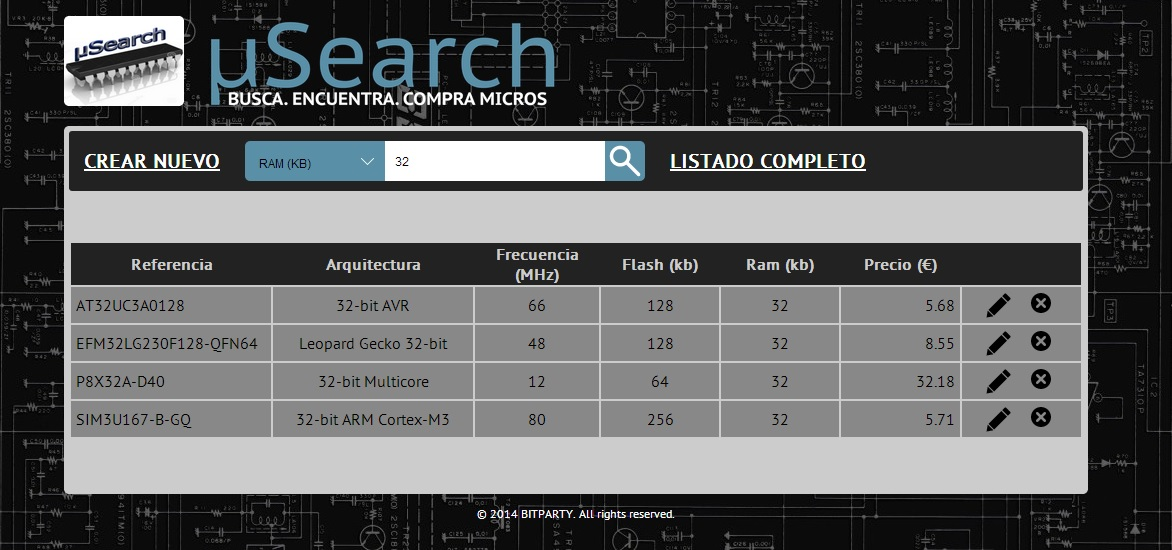
\includegraphics[width=0.70\textwidth]{img/listado_busqueda_admin}
	\caption{Página de listado de resultado de búsqueda.}
	\label{fig:listado_busqueda_admin}
\end{figure}

\paragraph{}Desde esta página, a través de los iconos situados en la cabecera debajo de los logotipos de la web, el administrador puede acceder a:

\begin{itemize}
	\item \textbf{Crear Nuevo:} Redirige al administrador a la página para añadir un nuevo microcontrolador al catálogo electrónico.

	\item \textbf{Búsqueda:} Desde esta sección de la cabecera, el administrador puede realizar de nuevo una búsqueda sobre el catálogo de microcontroladores en base a cualquiera de sus características (Arquitectura, Frecuencia, Flash, RAM). Se debe seleccionar una de las características de la lista despegable, introducir el texto a buscar y pulsar sobre el icono de búsqueda.
	El usuario será redirigido a una página donde se le mostrará el resultado de la búsqueda.
			
	\item \textbf{Listado Completo:} Redirige al administrador a la página en la que se listan todos los microcontroladores disponibles en el catálogo.
\end{itemize}